\section{سوال دوم}
در این سوال از الگوریتم ابتکاری مورچگان برای حل مسئله معروف فروشنده دوره‌گرد استفاده شده است. بخش
\ref{sec:part_I}
با فرض نبودن ترافیک،
بخش
\ref{sec:part_II}
با فرض ترافیک و بخش
\ref{sec:part_III}
با فرض اینکه ترافیک تابعی از زمان است حل شده است. در شکل
\ref{fig:cities}
مکان شهر‌ها رسم شده است.
\begin{figure}[H]
	\caption{مکان شهرها} 
	\centering 
	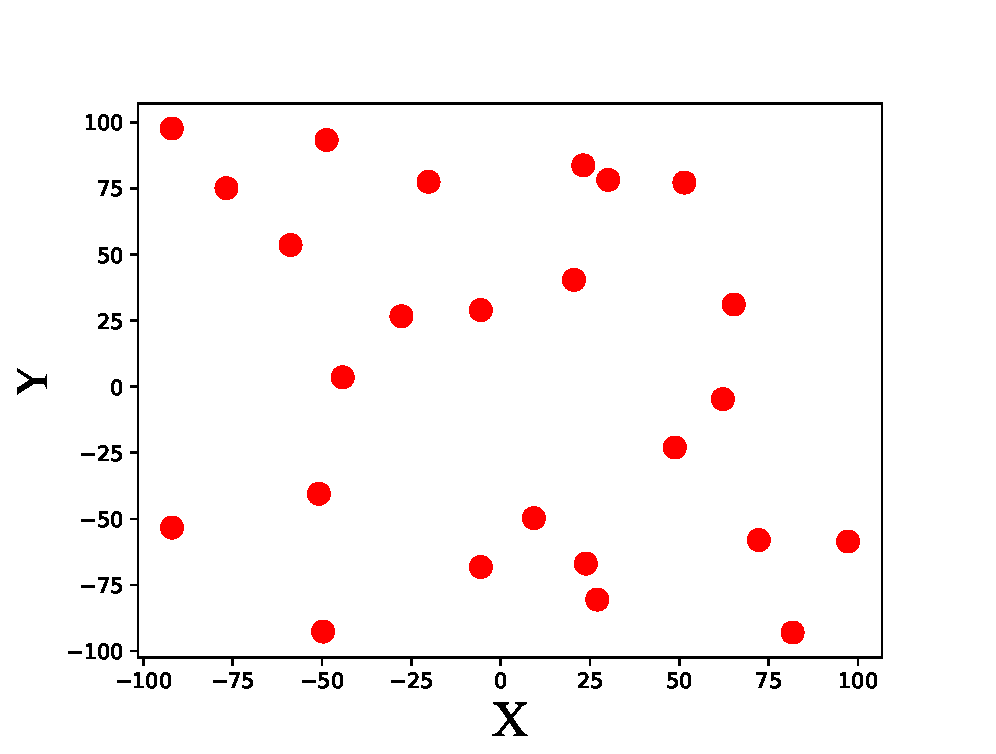
\includegraphics[width=16cm]{../Figure/Q2/Cities} 
	\label{fig:cities}
\end{figure}


در الگوریتم مورچگان ابتدا ماتریس فرمون برای هر مسیر تعریف می‌شود. با توجه به اینکه هیچ مورچه‌ای هنوز حرکت نکرده است، در ماتریس فرمون تعریف شده هر مسیر فرمون برابر با یک است. در ادامه هر مورچه برای انتخاب مسیر از احتمال زیر استفاده می‌کند.
\begin{equation}
	p_n(c_i, c_j) = \dfrac{\tau(c_i, c_j)^{\alpha}/\delta(c_i, c_j)^{\beta}}{\sum \tau(c_i, c_j)^{\alpha}/\delta(c_i, c_j)^{\beta}}
\end{equation}
که در رابطه بالا $\tau$ برابر با مقدار فرمون هر مسیر و $\delta$ برابر با طول مسیر است. بعد از آنکه تمامی مورچه‌ها حرکت کردند فرمون مسیر‌ها به صورت زیر به‌روز رسانی می‌شود.
\begin{equation}
	\tau(c_i, c_j) = (1-\rho)\tau(c_i, c_j) + \sum_{n=1}^{m} \Delta \tau(c_i, c_j) 
\end{equation}
که پارامتر رابطه بالا به صورت زیر تعریف می‌شود.
\begin{equation}
	\Delta \tau(c_i, c_j) = \dfrac{Q}{L}
\end{equation}
که در رابطه بالا $L$ برابر با طول مسیر طی شده توسط مورچه است. 
پارامتر $Q$ برای رفتار بهتر الگوریتم استفاده شده است.
پارامترهای الگوریتم مورچگان بر اساس اعداد رایج در مقاله‌ها انتخاب شده است. پارامترهای الگوریتم مورچگان در جدول
\ref{tab:ACO_pat}
آورده شده است.

\lr{\begin{table}[H]
		\caption{Parameter of ACO}
		\vspace{0.5cm}
		\centering
		\begin{tabular}{|c|c|c|}
			\hline
			\lr{Value} & \lr{Parameter}\\
			\hline
			10 & \lr{Number of Ants}\\
			100 & \lr{Number of Iterations}\\
			\hline
			1 & $\alpha$\\
			5 & $\beta$\\
			0.5 & $\rho$\\
			100 & $Q$\\
			\hline
		\end{tabular}
	\label{tab:ACO_pat}
\end{table}}

\subsection{پخش اول}\label{sec:part_I}
با توجه به اینکه الگوریتم مورد استفاده ابتکاری است و تابع رندوم بخش مهمی از آن است در اینجا دو راه حل (شکل های
\ref{fig:part_I_ACO_sol_1}
و 
\ref{fig:part_I_ACO_sol_2}
) آورده شده است. طول هر مسیر نیز در جدول \ref{tab:part_I_cost}
آورده شده است. برای حل این مسئله از یک ماتریس به اسم
\lr{graph}
 برای توصیف فاصله‌ی بین شهرها استفاده شده است

\begin{figure}[H]\label{fig:part_I_ACO_sol_1}
	\caption{راه حل اول تولید شده توسط الگوریتم ACO} 
	\centering 
	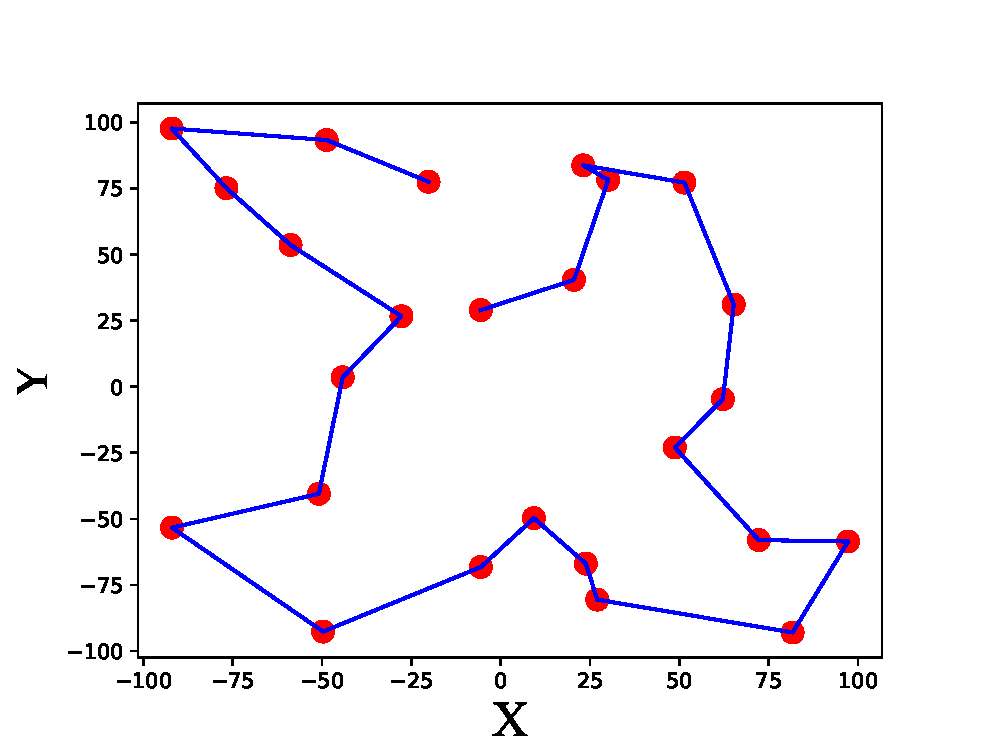
\includegraphics[width=16cm]{../Figure/Q2/ACO_solution} 
\end{figure}

\begin{figure}[H]\label{fig:part_I_ACO_sol_2}
	\caption{راه حل دوم تولید شده توسط الگوریتم ACO} 
	\centering 
	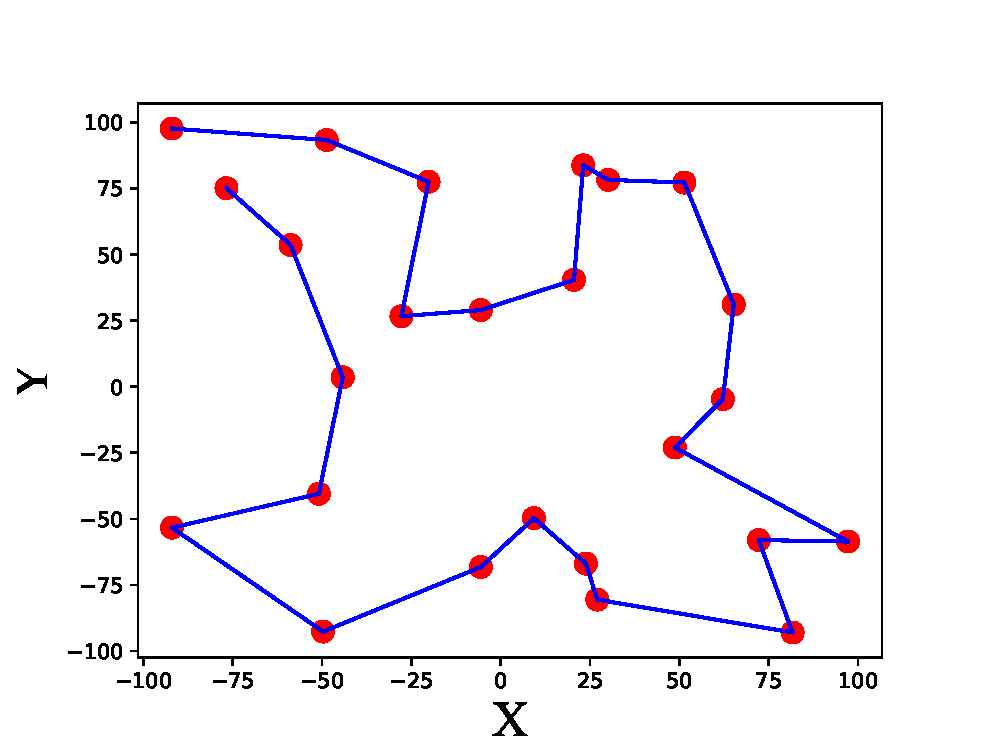
\includegraphics[width=16cm]{../Figure/Q2/ACO_solution_1} 
\end{figure}

\lr{\begin{table}[H]\label{tab:part_I_cost}
		\caption{Cost of solution produced with ACO}
		\vspace{0.5cm}
		\centering
		\begin{tabular}{|c|c|c|}
			\hline
			\lr{solution 2 Cost} & \lr{solution 1 Cost}\\
			\hline
			899.8 & 881.0\\
			\hline
		\end{tabular}
\end{table}}

\subsection{بخش دوم}\label{sec:part_II}

در بخش
\ref{sec:part_I}
ماتریس
\lr{graph}
معرفی شد. در این بخش برای اضافه کردن ترافیک، درایه‌های ماتریس
\lr{traffic}
به‌صورت نظیر به نظیر تقسیم بر درایه‌های ماتریس
\lr{graph}
(هر چه سرعت بیشتر باشد هزینه رفتن از شهر i به j کمتر است) می‌شوند.

\begin{figure}[H]
	\caption{راه حل تولید شده توسط الگوریتم ACO با در نظر گرفتن ترافیک} 
	\centering 
	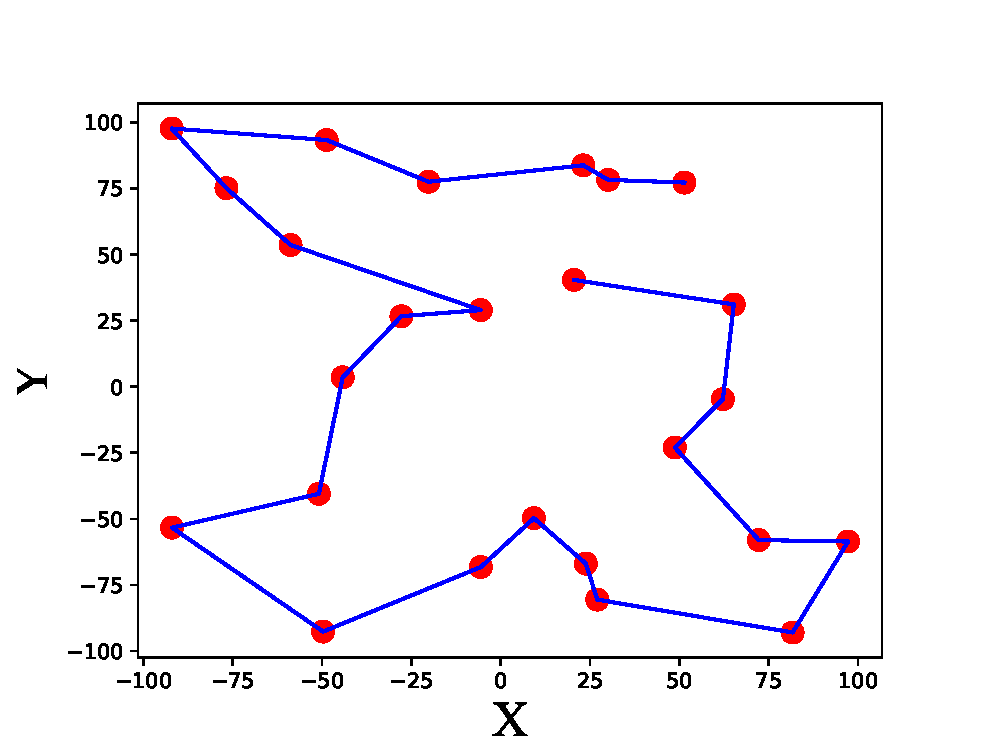
\includegraphics[width=16cm]{../Figure/Q2/ACO_traffic_solution} 
\end{figure}

\subsection{بخش سوم}\label{sec:part_III}
برای ترافیک متغیر با زمان دو رویکرد در نظر گرفته شد. رویکرد اول آن بود که در هر زمان مسئله از اول حل شود و رویکرد دوم به این صورت بود که در زمان بعدی فرمون زمان قبل باقی بماند ولی ترافیک مسیر عوض شده باشد. مقایسه نتایج دو رویکرد در جدول
\ref{tab:part_III_cost}
آورده شده است. برای پویانمایی مسیر بهینه دو فایل
\lr{gif}
با نام‌های
\lr{time\_varing\_traffic\_solution}
و
\lr{time\_varing\_traffic\_solution\_gph}
در پوشه 
\lr{Figure/Q2}
وجود دارد که هر کدام برای یک رویکرد اشاره شده است.

\lr{\begin{table}[H]\label{tab:part_III_cost}
		\caption{Cost of solution produced with ACO}
		\vspace{0.5cm}
		\centering
		\begin{tabular}{|c|c|c|}
			\hline
			\lr{global pheromone solution} & \lr{local pheromone solution} & \lr{Time}\\
			\hline
			879.96 & 874.72& \lr{i = 0}\\
			1571.60 & 1491.50& \lr{i = 1}\\
			1138.58 & 936.80& \lr{i = 2}\\
			1152.92 & 1130.20& \lr{i = 3}\\
			1095.87 & 1011.32& \lr{i = 4}\\
			1080.46 & 1030.46& \lr{i = 5}\\
			1357.68 & 1324.29& \lr{i = 6}\\
			1077.28 & 1081.62& \lr{i = 7}\\
			1163.53 & 1129.28& \lr{i = 8}\\
			1309.49 & 1329.87& \lr{i = 9}\\
			\hline
			11827.44 & 11340.11 & sum\\
			\hline
		\end{tabular}
\end{table}}



